%+----------------------------------------------------------------------------+
%| SLIDES: Phd Thesis - public Defence
%| Contents:	- 45 minutes (extimated duration 3 minutes per slide )
%|			 	- 20 minutes introductory slides, ~ 7 slides
%|			 	- 25 Techincal Slides.,~ 8 slides  
%|				- Backup Slides on technical points			
%|
%| Author: Antonio miti
%| Place: Milano, April 2021
%+----------------------------------------------------------------------------+


%- HandOut Flag -----------------------------------------------------------------------------------------
\newif\ifHandout
%	\Handouttrue  %uncomment for the printable version


%- D0cum3nt ----------------------------------------------------------------------------------------------
\ifHandout
	\documentclass[handout,10pt]{beamer}   
	\setbeameroption{show notes} %print notes   
\else
	\documentclass[10pt]{beamer}
\fi



%- Packages ----------------------------------------------------------------------------------------------
\usepackage{custom-style}
\usepackage{array}
\usepackage{pbox}

%--Beamer Style-----------------------------------------------------------------------------------------------
\usetheme{toninus}
\usepackage{animate}
\usetikzlibrary{positioning, arrows}
\usetikzlibrary{shapes,decorations}
\usetikzlibrary{backgrounds}
  \tikzset{
    invisible/.style={opacity=0},
    visible on/.style={alt=#1{}{invisible}},
    alt/.code args={<#1>#2#3}{%
      \alt<#1>{\pgfkeysalso{#2}}{\pgfkeysalso{#3}} % \pgfkeysalso doesn't change the path
    },
  }



%- T1tle P4g3 -------------------------------------------------------------------------------------------
\title{Homotopy comomentum maps \\ in Multisymplectic Geometry} 
\subtitle{\href{ttps://set.kuleuven.be/phd/sap/dualjoint/public}{Public Defence}}
\author[AMM]{\href{https://dmf.unicatt.it/miti/}{Antonio Michele Miti}}
\institute[UCSC and KU Leuven]{
  \begin{tabular}[h]{ccc}
      Università Cattolica del Sacro Cuore & $\qquad$ & KU Leuven \\
      Brescia, Italy & & Leuven, Belgium \\
      \href{https://dipartimenti.unicatt.it/dmf-home?rdeLocaleAttr=it}{\includegraphics[width=3.5cm]{./Logos/UnicattBS-logo}} & & 
      \href{https://wis.kuleuven.be/english}{\includegraphics[width=4cm]{./Logos/KULeuven_logo}}
  \end{tabular}      
}
\date[PublicDefence_21] % (optional, should be abbreviation of conference name)
{	
	\href{https://scuoledidottorato.unicatt.it/phdschools/science-home}{International Doctoral Programme in Science } \\
	{\vskip 1ex}
	April 1, 2021
}





\newcommand{\thankyouslide}[0]{
	\ifHandout

	\else
	\addtocounter{framenumber}{-1}
	\begin{frame}{}
	\label{frame:thankyouslide}
		\vfill
	  \centering 
	  {\Huge\color{red} 
	  \emph{Thank you for your attention!}}
		\vfill
		%
		\centering
		\begin{columns}
			\hfill
			\begin{column}{0.05\linewidth}
				\centering \includegraphics{beamericonarticle}
			\end{column}
			\begin{column}{0.8\linewidth}
				\centering
				\textbf{On some (multi)symplectic aspects of link invariants},
				\\
				\emph{AMM, Mauro Spera}, \href{https://arXiv.org/abs/1805.01696}{arxiv:1805.01696};\\
				(to appear in \emph{Journal of the Australian Mathematical Society})	
			\end{column}
			\begin{column}{0.05\linewidth}
				\centering \includegraphics{beamericonarticle}			
			\end{column}
			\hfill
		\end{columns}
		\vfill
		\begin{columns}
			\hfill
			\begin{column}{0.05\linewidth}
				\centering \includegraphics{beamericonarticle}
			\end{column}
			\begin{column}{0.8\linewidth}
				\centering
				\textbf{Multisymplectic actions of compact Lie groups on spheres},
				\\
				\emph{AMM, Leonid Ryvkin}, \href{https://arxiv.org/abs/1906.08790}{arXiv:1906.08790};
				\\
				(to appear in \emph{Journal of Symplectic Geometry})
			\end{column}
			\begin{column}{0.05\linewidth}
				\centering \includegraphics{beamericonarticle}			
			\end{column}
			\hfill
		\end{columns}		
		\vfill		
		\begin{columns}
			\hfill
			\begin{column}{0.05\linewidth}
				\centering \includegraphics{beamericonarticle}
			\end{column}
			\begin{column}{0.8\linewidth}
				\centering
		\textbf{Derivation of the HOMFLYPT knot polynomial via helicity and geometric quantization},
				\\
		\emph{AMM, Mauro Spera}, \href{https://arxiv.org/abs/1910.13400}{arXiv:1910.13400};\\
				(to appear in \emph{Bollettino dell'Unione Matematica Italiana})	
			\end{column}				
			\begin{column}{0.05\linewidth}
				\centering \includegraphics{beamericonarticle}			
			\end{column}
			\hfill
		\end{columns}
		\vfill
		\begin{columns}
			\hfill
			\begin{column}{0.05\linewidth}
				\centering \includegraphics{beamericonarticle}
			\end{column}
			\begin{column}{0.8\linewidth}
				\centering
				\textbf{Observables of multisymplectic manifolds and higher Courant algebroids},
				\\
				\emph{AMM, Marco Zambon}; % \href{https://arXiv.org/abs/1805.01696}{arxiv:1805.01696};\\
				(To appear soon on \emph{arxiv})	
			\end{column}
			\begin{column}{0.05\linewidth}
				\centering \includegraphics{beamericonarticle}			
			\end{column}
			\hfill
		\end{columns}
	\end{frame}
	\note[itemize]{
		\item
	}
	\fi
}






%---------------------------------------------------------------------------------------------------------------------------------------------------
%- D0cum3nt ----------------------------------------------------------------------------------------------------------------------------------
\begin{document}
%-------------------------------------------------------------------------------------------------------------------------------------------------
\begin{frame}  % Alternative: \maketitle outside of frame
	\titlepage
	\ifHandout
		\tikz[overlay,remember picture]
		{
	    	%	\node at ($(current page.west)+(1.5,0)$) [rotate=90] {\Huge\textcolor{gray}{\today}};
	    	\node[        
	    		draw,
	    		shape border rotate=90,
			isosceles triangle,
			isosceles triangle apex angle=90,
			fill=yellow]
	        		at ($(current page.north east)-(1,1)$) [rotate=-45] {\textcolor{red}{Handout version}};
		}
	\fi
	\end{frame}
	\addtocounter{framenumber}{-1}
\note{
	%Abstract?
	\textbf{\underline{OUTLINE}}:
	\tableofcontents
}
%---------------------------------------------------------------------------------------------------------------------------------------------------
\outline




%-------------------------------------------------------------------------------------------------------------------------------------------------
\section{Introduction}
%-------------------------------------------------------------------------------------------------------------------------------------------------

%-------------------------------------------------------------------------------------------------------------------------------------------------
\begin{frame}[fragile]{Keywords}
\tikzstyle{every picture}+=[remember picture]
	
	\begin{columns}
    	\begin{column}{.45\textwidth}
		 \tikz[baseline]{
		            \node[visible on=<5->,draw=orange!80,anchor=base,text width=5.5cm] (s1)
		            {Adjectives implying a certain \\ 
		            \emph{higher generalization}.};
			}    	
		\end{column}
    	\begin{column}{.45\textwidth}
		 \tikz[baseline]{
		            \node[visible on=<4->,draw=blue!80,anchor=base, text width=5.5cm] (s2)
		            {An auxiliary mathematical object possesed by symmetries \\
		            \emph{= group of transformations preserving the symplectic structure.}};
			}       	
		\end{column}
	\end{columns}

	\begin{center}
		\large
		 \tikz[baseline]{
		            \node[fill=orange!20,anchor=base] (t1)
		            {Homotopy};
			}
		 \tikz[baseline]{
		            \node[fill=blue!20,anchor=base] (t2)
		            {comomentum maps};
		        } 
		\\
		in 
		 \tikz[baseline]{
	            \node[fill=orange!20,anchor=base] (t5)
	            {multi -};
		}
		 \tikz[baseline]{
	            \node[fill=red!20,anchor=base] (t3)
	            {symplectic};
		}		
		\tikz[baseline]{
	            \node[fill=green!20,anchor=base] (t4)
	            {geometry};
		}	
	\end{center}

	\begin{columns}
    	\begin{column}{.45\textwidth}
 		 \tikz[baseline]{
	            \node[visible on=<3->,draw=red!80,anchor=base,text width=5.5cm] (s3)
	            {Geometric structure prescribing how to measure the area of 2-dimensional surface elements embedded in the manifold.};
		}		   	
		\end{column}
    	\begin{column}{.45\textwidth}
		\tikz[baseline]{
	            \node[visible on=<2->,draw=green!80,anchor=base,text width=5.5cm] (s4)
	            {Differential geometry: \\
	            	the study of smooth manifolds \\
	            	\emph{= generalized surfaces (possible dimension greater then two) that can be charted}.
	            };
		}	
		\end{column}
	\end{columns}

	\begin{tikzpicture}[overlay]
        \path[visible on=<5->,->,orange!80] (s1) edge [bend right] (t1);
        \path[visible on=<4->,->,blue!80] (s2) edge [bend left] (t2);
        \path[visible on=<3->,->,red!80] (s3) edge [bend right] (t3);
        \path[visible on=<2->,->,green!80] (s4) edge [bend right] (t4);
        \path[visible on=<5->,->,orange!80] (s1) edge [bend right] (t5);
	\end{tikzpicture}

	\vfill
	\onslide<6->{
		\begin{center}
			\large
			\bf
			Framework: \alert{\emph{Geometric Mechanics}}
		\end{center}
	}
	
	
	
\end{frame}
\note[itemize]{
	\item dare una vaga idea dei termini del titolo
	\item indicare il contesto in cui è possibile inquadrare la tesi. framewor: geometric mechanics
}
%-------------------------------------------------------------------------------------------------------------------------------------------------

%-------------------------------------------------------------------------------------------------------------------------------------------------
\begin{frame}[t,fragile]{What is... mechanics?}
	\begin{center}
		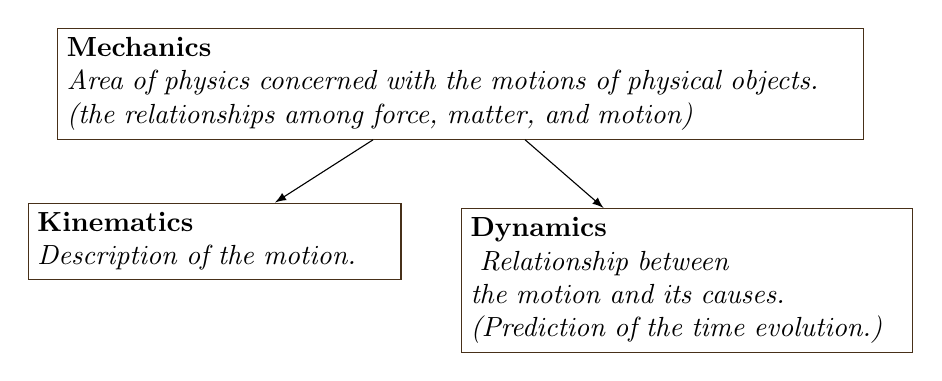
\begin{tikzpicture}
		 	\node[draw=orange!20!black!90,right,text width=10cm] (s1) at (0,0)
		    {
				{\bf Mechanics} \\
				\emph{Area of physics concerned with the motions of physical objects.\\
				(the relationships among force, matter, and motion)}		            
		     }; 
 			\node[draw=orange!20!black!90,text width=4.5cm] (t1) at (2cm,-2cm)
    		{
		   		{\bf Kinematics}
		   		\\ \emph{Description of the motion.}
	        };	
 			\node[draw=orange!20!black!90,text width=5.5cm] (t2) at (8cm,-2.5cm)
    			{
		    		{\bf Dynamics} \\
		   			\emph{ Relationship between\\ the motion and its causes.\\ (Prediction of the time evolution.)}
	        };
	        \draw[-latex] (s1) -- (t1);
        	\draw[-latex] (s1) -- (t2);
		\end{tikzpicture}
	\end{center}

	\vfill
	\begin{columns}
    	\begin{column}{.33\textwidth}
	   		\includegraphics[width=\textwidth]{Pictures/solar} 	
		\end{column}
    	\begin{column}{.33\textwidth}
	   		\includegraphics[width=\textwidth]{Pictures/autogru-liebherr} 	
		\end{column}
    	\begin{column}{.33\textwidth}
	   		\includegraphics[width=\textwidth]{Pictures/plasma} 	
		\end{column}
	\end{columns}
\end{frame}
\note[itemize]{
	\item
}
%-------------------------------------------------------------------------------------------------------------------------------------------------

%-------------------------------------------------------------------------------------------------------------------------------------------------
\begin{frame}[t]{How does Geometry gets into Physics?}
	%
	\begin{block}{Trivial answer:}
		It appears in describing the "physical space" in which all "physical systems" are embedded.
	\end{block}
	\vfill
  	\begin{columns}<2->[T]
    	\begin{column}{.45\textwidth}
    		\begin{center}
				\includegraphics[width=0.9\textwidth]{Pics/map} 		
    		\end{center}
    	\end{column}
    	\begin{column}{.55\textwidth}
    		\vspace*{1em}
			\begin{block}{Historical fact:}
				Modern (intrinsic) differential geometry stemmed from a cartographic survey of the Kingdom of Hanover commissioned to Carl Friederich Gauss in 1828.		
			\end{block}
    	\end{column}
    \end{columns}
	\vfill
	\begin{alertblock}<3->{There is much more!}
		Geometry provides a powerful language to encode deep properties of physics encompassing a huge variety of mechanical systems.
	\end{alertblock}
\end{frame}
\note[itemize]{
	\item Three fundamentals concepts: Space, Body (system), Displacement.
	\item Nevertheless, the problem of measuring "Earth" is one of the oldest problem in mathematics (see \url{https://en.wikipedia.org/wiki/YBC_7289})
	\item Nel 1818 fu chiesto a Gauss di compiere la rilevazione geodetica del Regno di Hannover, associandola ai precedenti rilevamenti effettuati in Danimarca.
La cartografia dell'Hannover portò Gauss a sviluppare la geometria differenziale insieme alle potenzialità della geometria non euclidea.
}
%-------------------------------------------------------------------------------------------------------------------------------------------------

%-------------------------------------------------------------------------------------------------------------------------------------------------
\begin{frame}{What we mean by: \emph{Geometric mechanics}? (1)}
	\alert{"Geometric mechanics" is not a completely standard (widely accepted) term.} \\
	It needs some clarification...
	\vfill
	\pause
	The idea of intermarrying geometry with mechanics has a noble father...
	\begin{columns}[T]
		\begin{column}{.4\textwidth}
			\center
			\includegraphics[width=0.8\textwidth]{Pictures/FFat/Galileo} 
		\end{column}
		\begin{column}{.6\textwidth}
			\only<2>{
			\begin{quotation}
			{\footnotesize 
				«La filosofia è scritta in questo grandissimo libro che continuamente ci sta aperto innanzi a gli occhi (io dico {\bf l'universo}), ma non si può intendere se prima non s'impara a intender la lingua, e conoscer i caratteri, ne' quali è scritto. 
				Egli {\bf è scritto in lingua matematica, e i caratteri son triangoli, cerchi, ed altre figure geometriche}, senza i quali mezzi è impossibile a intenderne umanamente parola; senza questi è un aggirarsi vanamente per un oscuro laberinto.»
			}
			\end{quotation}
			}
			\only<3->{		
			\begin{quotation}
			{\footnotesize 
				«Philosophy {\bf [nature]} is written in that great book which ever is before our eyes -- I mean the universe -- but we cannot understand it if we do not first learn the language and grasp the symbols in which it is written. 
				The book {\bf is written in mathematical language, and the symbols are triangles, circles and other geometrical figures}, without whose help it is impossible to comprehend a single word of it; without which one wanders in vain through a dark labyrinth.»		
			}
			\end{quotation}	
			}
			(Galileo Galilei, Il Saggiatore, 1623)	
		\end{column}	
	\end{columns}	
\end{frame}
\note[itemize]{
	\item Praticamente l'idea è vecchia quanto la scienza.f
}
%-------------------------------------------------------------------------------------------------------------------------------------------------


%-------------------------------------------------------------------------------------------------------------------------------------------------
\begin{frame}{What we mean by: \emph{Geometric mechanics}? (2)}
	What we mean \underline{here} is:
	\\
	the modern discipline originated in the 60s by the work of these mathematicians%gentlemen
	
	\vfill
	\begin{columns}[T]
		\begin{column}{.2\textwidth}
			\center
			\includegraphics[width=0.8\textwidth]{Pictures/FFat/arnold}
			Vladimir \\ 
			Arnold
		\end{column}
		\begin{column}{.2\textwidth}
			\center
			\includegraphics[width=0.8\textwidth]{Pictures/FFat/souriau} 
			Jean-Marie \\			
			Souriau
		\end{column}
		\begin{column}{.2\textwidth}
			\center
			\includegraphics[width=0.8\textwidth]{Pictures/FFat/smale}
			Stephen \\
			Smale
		\end{column}
		\begin{column}{.2\textwidth}
			\center
			\includegraphics[width=0.8\textwidth]{Pictures/FFat/abraham} 
			Ralph \\			
			Abraham
		\end{column}
		\begin{column}{.2\textwidth}
			\center
			\includegraphics[width=0.8\textwidth]{Pictures/FFat/marsden} 
			Jerrold \\
			Marsden
		\end{column}		
	\end{columns}	

	\pause
	\vfill
	\begin{block}<1->{Introduced as a branch of \emph{(applied) Mathematics}}
			Employs modern (differential) geometry to the description of dynamical systems.	
	\end{block}


\end{frame}
\note[itemize]{
	\item %\href{https://en.wikipedia.org/wiki/Geometric_mechanics#History}{wiki}
		Arnold's fundamental work showed that Euler's equations for the free rigid body are the equations for geodesic flow on the rotation group SO(3) and carried this geometric insight over to the dynamics of ideal fluids, where the rotation group is replaced by the group of volume-preserving diffeomorphisms. 
	\item Smale's paper on Topology and Mechanics investigates the conserved quantities arising from Noether's theorem when a Lie group of symmetries acts on a mechanical system, and defines what is now called the momentum map (which Smale calls angular momentum), and he raises questions about the topology of the energy-momentum level surfaces and the effect on the dynamics. 
	\item Souriau also considered the conserved quantities arising from the action of a group of symmetries, but he concentrates more on the geometric structures involved (for example the equivariance properties of this momentum for a wide class of symmetries), and less on questions of dynamics.
	\item These ideas leads to the seminal book: \emph{Foundations of Mechanics} by Abraham and Marsden (1978).
	\item 		{physical è un po' restrittivo, diciamo sistemi che evolvono?}	
		{dynamical systems: non solo meccanica classica non relativistica non quantistica!}

}
%-------------------------------------------------------------------------------------------------------------------------------------------------

%-------------------------------------------------------------------------------------------------------------------------------------------------
\begin{frame}[t]{What is... \emph{Geometric Mechanics?}}
		\begin{block}{As an approach to \emph{Rational Mechanics}:}
			\begin{itemize}
				\item \textbf{Key idea:} make use of geometry to completely encode a physical system's mechanical properties regardless of the coordinate system employed.
				\item \textbf{The goal:} reconstruction of the physical observable quantities of interest from these abstract mathematical setting.
				\item \textbf{Advantage:} formalize the system's relevant structure in order to:
					\begin{itemize}
						\item[-] simplify the analytical or numerical solution of motion equations;
						\item[-] derive its quantum or relativistic counterpart.		
					\end{itemize}									
			\end{itemize}
		\end{block}
		%
		\vfill
		\pause
		\begin{block}{Some direct applications:}
			\vspace{-0.5em}
			\begin{columns}
		    	\begin{column}{.45\textwidth}
					\begin{itemize}
						\item[-] Theoretical chemistry
						\item[-] Control theory
						\item[-] Image processing
					\end{itemize}
				\end{column}
		    	\begin{column}{.45\textwidth}
					\begin{itemize}
						\item[-] Mathematical finance
						\item[-] Earth sciences
						\item[-] Robotics
					\end{itemize}
				\end{column}
			\end{columns}
		\end{block}
		\vfill
		\pause
		\begin{block}{Three cornerstones of geometric mechanics}
	\begin{center}
		%\scalebox{.8}{%
		{
		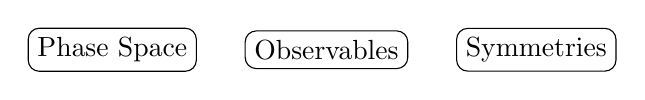
\begin{tikzpicture}[>=stealth,every node/.style={shape=rectangle,draw,rounded corners},node distance=0.05\linewidth,]
	    % create the nodes
		    \node (a1) {Phase Space};
		    \node (a2)[right =of a1] {Observables};
		    \node (a3)[right =of a2] {Symmetries};
		\end{tikzpicture}
%				\node [text width=0.6\linewidth, rectangle,draw,right of=lhs] (rhs) {Lie subgroup \\$G \subset Diff(M)$};
		}			
	\end{center}		
		\end{block}


		%https://en.wikipedia.org/wiki/Geometric_mechanics

		%http://www10.mathematik.uni-wuerzburg.de/index.php?path=research/maphy
	\end{frame}
	\note[itemize]{
		\item the geometric language permits to formalize the evolution of system composed of both quantum and classical degree of freedom (mesoscopic scale)
		\item Lessig: 
		In our discussion we only considered classical mechanical systems. However,
the theory applies to a diverse array of fields and disciplines ranging from quantum mechanics at the smallest scales to relativistic astrophysics at the largest, and applications can be found in areas such as image processing, space mission design, marine animal propulsion, mathematical finance, rising eggs, oceanography, plasma physics, falling cat phenomena, and many more. In its contemporary formulation using the rich toolbox of modern geometry, geometric mechanics provides thereby a surprisingly unified perspective on all these systems.
		\item Manifolds arise naturally in the description of classical mechanical systems.
		\item Geometrization of mechanics yields an inherent intuition to differential geometry structures (manifolds, charts, vectors ...).
		\item Encoding a classical mechanical system via a precise mathematical framework allows  to the relevant structures of our physical theories to emerge.
		\item A sound mathematical foundation provides a solid ground where to perform axiomatization of physical theories, quantization and "relativization".
		\item With a slight refinement of the mathematical language, also systems with continuous degrees of freedom (fluid and fields) can be accommodated within this geometrical framework as well.
		\item This framework could be adapted directly to ordinary quantum mechanical systems (e.g. Bloch sphere).
		\item There are also  direct applications!!! (if you are that kind of person .... :P )
				(if aiming to a complete mathematical foundation it's not enough for you...)
	}
%-------------------------------------------------------------------------------------------------------------------------------------------------




%-------------------------------------------------------------------------------------------------------------------------------------------------

%-------------------------------------------------------------------------------------------------------------------------------------------------
\subsection{Phase Space}
\subcheckpoint	
%-------------------------------------------------------------------------------------------------------------------------------------------------
	\input{defence-configspace}
	%- HandOut Flag -----------------------------------------------------------------------------------------
\newif\ifHandout

%- D0cum3nt ----------------------------------------------------------------------------------------------
\documentclass[beamer,10pt]{standalone}   
%\documentclass[beamer,10pt,handout]{standalone}  \Handouttrue  

%- HandOut Flag -----------------------------------------------------------------------------------------
\ifHandout
	\setbeameroption{show notes} %print notes   
\fi

	
%- Packages ----------------------------------------------------------------------------------------------
\usepackage{custom-style}
\usetikzlibrary{positioning}
\usepackage{multicol}


%--Beamer Style-----------------------------------------------------------------------------------------------
\usetheme{toninus}
\usepackage{animate}
\usetikzlibrary{positioning, arrows}
\usetikzlibrary{shapes}
\usepackage{ifthen}

\begin{document}
%-------------------------------------------------------------------------------------------------------------------------------------------------
\begin{frame}{Phase Space}
\begin{columns}[T]
	\begin{column}{0.5\textwidth}
		\begin{center}
			\resizebox{\textwidth}{!}{		
				\pgfmathtruncatemacro\steps{50}
				\pgfmathtruncatemacro\maxtheta{30}
				\pgfmathtruncatemacro\pi{3.14}
				\begin{animateinline}[autoplay,loop]{10} % 5 fps, same as 0.2 s transduration
				  \multiframe{\steps}{i=0+1}{
				    \begin{tikzpicture}
				    \pgfmathsetmacro\fraction{\i/(\steps-1)}
					\pgfmathsetmacro\theta{\maxtheta*cos(360*\fraction)-90}
					\pgfmathsetmacro\v{-1*sin(360*\fraction)}
				
				    %frame
				    \draw[draw=none] (-6,-8) rectangle (6,6);		
					% Support
					\coordinate (o) at (0,0);
					\node[cross out,draw,black!10] (0,0){};
					\node[circle,draw,black!10] (0,0){};
					% Bob's trajectory
					\draw[blue,line width=1mm] (0,0) circle (4);
					% Rod + Bob
					\draw[dashed] (0,0) -- (\theta:4) node[fill,circle,red](m){};

					% Velocity
					\ifthenelse{\equal{\i}{0}}
           			{}
           			{\draw[-latex,green!80!black,line width=1mm] (m) -- node[green!80!black,below right]{$\vec{v}$}($(m)!\v!-90:(o)$);}
				    \end{tikzpicture}
				  }
				\end{animateinline}
			}
		\end{center}
	\end{column}
	\begin{column}{0.5\textwidth}
		\begin{itemize}
			\item Knowing the position is not sufficient to determine the evolution of the system.
			\item (Displacement encode statics, one must know how configurations evolves in time)
			\item One needs to know also the velocity (or better, the momentum).
		\end{itemize}

		\vspace{1em}
		\onslide<2->{
			\begin{upshotblocksimp}
				Upshot:
				Configurations $\neq$ \emph{States}
			\end{upshotblocksimp}			
		}
	\end{column}
\end{columns}
\end{frame}
\note[itemize]{
	\item
}
%-------------------------------------------------------------------------------------------------------------------------------------------------

%-------------------------------------------------------------------------------------------------------------------------------------------------
\begin{frame}{Phase Space}
\begin{columns}[T]
	\begin{column}{0.5\textwidth}
		\begin{center}
			\resizebox{\textwidth}{!}{
				\begin{tikzpicture}
					\node[draw=none] (o) at (0, 0) {o};
				    %frame
				    \draw[draw=none] (-6,-8) rectangle (6,6);				
					\draw[draw=none](0,0)--(-90:4)node[circle, fill, minimum size=5pt,
				              inner sep=0pt, outer sep=0pt](p){};
					\draw[green,line width=1mm] ($ (p)!3.5cm!90:(o) $) -- ($ (p)!3.5cm!270:(o) $);
					\draw[green,dashed,line width=1mm] ($ (p)!4.5cm!90:(o) $) -- ($ (p)!4.5cm!270:(o) $);
					\draw[blue,line width=1mm] (0,0) circle (4);
				\end{tikzpicture}
			}
			%
		\end{center}
	\end{column}
	\begin{column}{0.5\textwidth}
 		\begin{itemize}
 			\item consider {\bf a} configuration.
 			\item all possible velocities are encoded by points on the tangent line at the given configuration \\(\emph{Tangent space}).
 		\end{itemize}
	\end{column}
\end{columns}
\end{frame}
\note[itemize]{
	\item
}
%-------------------------------------------------------------------------------------------------------------------------------------------------

%-------------------------------------------------------------------------------------------------------------------------------------------------
\begin{frame}{Phase Space}
\begin{columns}[T]
	\begin{column}{0.5\textwidth}
		\begin{center}
			\only<1>{
			\resizebox{\textwidth}{!}{
				\begin{tikzpicture}
					\node[draw=none] (o) at (0, 0) {o};
				    %frame
				    \draw[draw=none] (-6,-8) rectangle (6,6);						
					\foreach \x in {0,30,...,360}{
						\draw[draw=none](0,0)--(\x:4)node[circle, fill, minimum size=5pt,
					              inner sep=0pt, outer sep=0pt](p){};
					\draw[green,line width=1mm] ($ (p)!3.5cm!90:(o) $) -- ($ (p)!3.5cm!270:(o) $);
					\draw[green,dashed,line width=1mm] ($ (p)!4.5cm!90:(o) $) -- ($ (p)!4.5cm!270:(o) $);
					}
						\draw[blue,line width=1mm] (0,0) circle (4);
				\end{tikzpicture}
			}}
			%
			\only<2->{
			\resizebox{.7\textwidth}{!}{
				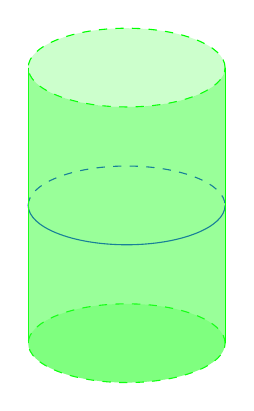
\begin{tikzpicture}
					\draw[green,dashed,fill=green!20] (0,0) ellipse (1.25 and 0.5);
					\draw [blue](-1.25,-1.75) arc (180:360:1.25 and 0.5);
					%\draw [blue,dashed] (-1.25,-3.5) arc (180:360:1.25 and -0.5);
					\draw[green,dashed,fill=green!20] (0,-3.5) ellipse (1.25 and 0.5);
					\draw [blue,dashed] (-1.25,-1.75) arc (180:360:1.25 and -0.5);
					\draw [green](-1.25,0) -- (-1.25,-3.5);
					\draw [green](1.25,-3.5) -- (1.25,0);  
					\fill [green!80,opacity=0.5] (-1.25,0) -- (-1.25,-3.5) arc (180:360:1.25 and 0.5) -- (1.25,0) arc (0:180:1.25 and -0.5);
				\end{tikzpicture}		
%				\begin{tikzpicture}
%				  \node[cylinder,draw=black,thick,aspect=0.7,minimum height=4cm,minimum width=2.5cm,shape border rotate=90,cylinder uses custom fill, cylinder body fill=green!30,cylinder end fill=green!10] (A) {\phantom{A}};
%				  \draw[dashed]
%				    let \p1 = ($ (A.after bottom) - (A.before bottom) $),
%				        \n1 = {0.5*veclen(\x1,\y1)-\pgflinewidth},
%				        \p2 = ($ (A.bottom) - (A.after bottom)!.5!(A.before bottom) $),
%				        \n2 = {veclen(\x2,\y2)-\pgflinewidth}
%				  in
%				    ([xshift=-\pgflinewidth] A.before bottom) arc [start angle=0, end angle=180,
%				    x radius=\n1, y radius=\n2];
%				\end{tikzpicture}	
}
			}
		\end{center}
	\end{column}
	\begin{column}{0.5\textwidth}
		\vspace{1.5em}
 		\begin{itemize}
 			\item Consider {\bf all possible} configurations.
 			\item Collect all possible pairs of position/momentum.
 			%\item points on the \emph{Tangent space}
 		\end{itemize}
		\vspace{1.5em} 		
 		\begin{itemize}
 			\item<2-> joining together all "tangent" space in a smooth and non-overlapping manner...
 		\end{itemize}
		\only<3->{
			\begin{upshotblocksimp}
				Upshot:
				We get another manifold (\emph{vector bundle}).
			\end{upshotblocksimp}					
		} 		
	\end{column}
\end{columns}
\end{frame}
\note[itemize]{
	\item  		
 		Collect all possible pair of position and momentum
 		
 		Informally, the tangent bundle of a manifold (which in this case is a circle) is obtained by considering all the tangent spaces (top), and joining them together in a smooth and non-overlapping manner (bottom).

}
%-------------------------------------------------------------------------------------------------------------------------------------------------

%-------------------------------------------------------------------------------------------------------------------------------------------------
\begin{frame}{Phase Space}
\begin{columns}[T]
	\begin{column}{0.5\textwidth}
		\begin{center}
			\includegraphics[width=\textwidth]{Pictures/pendo-phasespace}
		\end{center}
	\end{column}
	\begin{column}{0.5\textwidth}
 		\begin{itemize}
 			\item Consider {\bf all possible} configurations.
 			\item Collect all possible pairs of position/momentum.
 		\end{itemize}
		
		\vspace{1em}		
		\begin{defblock}[Phase Space]
			\begin{itemize}
				\item[=] collection of all \emph{states}
				\item[=] set of every possible "initial datas" (sufficient to reconstruct the motion).
			\end{itemize}
		\end{defblock}

		\vspace{1em}				
		\begin{mathblock}
			The Phase space is a \underline{symplectic} smooth manifold $(M)$.
		\end{mathblock}		
		
	\end{column}
\end{columns}
\end{frame}
\note[itemize]{
	\item You get an infinite cylinder (in the case of bipendulum I cannot picture it because we go directly into more than 2 dimensions.
	\item ho disegnato due traiettori sul fase space per mostrare come due natural motions si possono rappresentare bene qui sopra.
	\item per capire il significato di dell'aggettivo simplettico dobbiamo introdurre qualche altro interprete.

}
%-------------------------------------------------------------------------------------------------------------------------------------------------


\end{document}


%-------------------------------------------------------------------------------------------------------------------------------------------------
\subsection{Observables and time evolution}
\subcheckpoint	
%-------------------------------------------------------------------------------------------------------------------------------------------------
	%- HandOut Flag -----------------------------------------------------------------------------------------
\makeatletter
\@ifundefined{ifHandout}{%
  \expandafter\newif\csname ifHandout\endcsname
}{}
\makeatother

%- D0cum3nt ----------------------------------------------------------------------------------------------
\documentclass[beamer,10pt]{standalone}   
%\documentclass[beamer,10pt,handout]{standalone}  \Handouttrue  

\ifHandout
	\setbeameroption{show notes} %print notes   
\fi

	
%- Packages ----------------------------------------------------------------------------------------------
\usepackage{custom-style}
\usetikzlibrary{positioning}
\usepackage{multicol}


%--Beamer Style-----------------------------------------------------------------------------------------------
\usetheme{toninus}
\usepackage{animate}
\usetikzlibrary{positioning, arrows}
\usetikzlibrary{shapes,shapes.callouts}

\begin{document}

%-------------------------------------------------------------------------------------------------------------------------------------------------
\begin{frame}{Observables}
	An observables is:
	\vfill
	\begin{columns}[T]
		\begin{column}{0.5\textwidth}
			\begin{itemize}
				\item a procedure to read a certain quantity (a number) out of any state of the system
				\item<2-> a quantity that can be measured with a device. 
			\end{itemize}				
			%
			\vspace{.5em}
			\onslide<3->{
				\begin{exblock}[Pendulum inclination]
					Measure the inclination of the rod with a goniometer.
				\end{exblock}			
			}
			%
			\vspace{.5em}
			\onslide<4->{
				\begin{mathblock}
					Observables are given by smooth functions on the phase space $M$:
					\begin{displaymath}
						\mathcal{O}=C^{\infty}(M)~.
					\end{displaymath}
				\end{mathblock}
			}
		\end{column}
		\begin{column}{0.5\textwidth}
			\begin{center}
				\includegraphics<1>[width=.9\textwidth]{Pictures/pendo60-nogonio}
				\includegraphics<2>[width=.9\textwidth]{Pictures/pendo60}
				\includegraphics<3>[width=.9\textwidth]{Pictures/observo}
				\only<3>{
					\tikz[overlay,remember picture]
					{
						\node[ellipse callout,fill=white!50,
			               draw=black,
			               anchor=base]            
			            	 (base) at ($(current page.east)+(-5,3)$) [rotate=-0,text width=1.5cm,align=center,callout relative pointer={(-.3,-.8)}] 
			            	 {Measure: \\$\theta=\pi/3$\\$\phantom{\theta}\cong 1.05$};
					}	
				}
				\only<4>{
					\resizebox{.9\textwidth}{!}{				
						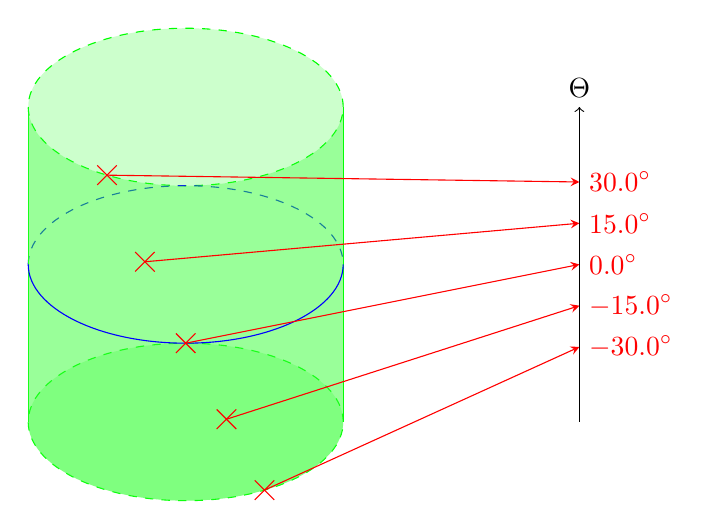
\begin{tikzpicture}
							\pgfmathtruncatemacro\steps{4}
							\pgfmathtruncatemacro\mintheta{-120}
							\pgfmathtruncatemacro\maxtheta{-60}
							\pgfmathsetmacro\deltatheta{(\maxtheta-\mintheta)/(\steps)}
							\pgfmathsetmacro\viewpitch{30}
							\pgfmathsetmacro\diam{2}
							\pgfmathsetmacro\H{4}
							\pgfmathsetmacro\deltaH{(\H)/(\steps)}
							\pgfmathsetmacro\X{\diam}
							\pgfmathsetmacro\Y{\diam*sin(\viewpitch)}	
							\pgfmathsetmacro\vel{\diam/4}	
		
							\draw[green,dashed,fill=green!20] (0,0) ellipse ({\X} and {\Y});
							%\draw [blue,dashed] (-1.25,-3.5) arc (180:360:1.25 and -0.5);
							\draw[green,dashed,fill=green!20] (0,-{\H}) ellipse ({\X} and {\Y});
							\draw [blue,dashed] (-{\X},-{.5*\H}) arc (180:360:{\X} and -{\Y});
							\draw [green](-{\X},0) -- (-{\X},-{\H});
							\draw [green]({\X},-{\H}) -- ({\X},0);  
							\fill [green!80,opacity=0.5] (-{\X},0) -- (-{\X},-{\H}) arc (180:360:{\X} and {\Y}) -- ({\X},0) arc (0:180:{\X} and -{\Y});
							\draw [blue](-\X,-{.5*\H}) arc (180:360:{\X} and {\Y});

							\foreach \i in {0,1,...,\steps}{
								\pgfmathsetmacro\h{-\i*\deltaH}
								\pgfmathsetmacro\theta{\mintheta + \i*\deltatheta}	
								\pgfmathsetmacro\thetalabel{-\theta -90}	
									
								\draw[red,-stealth] (0,\h)++({cos(\theta)*\X},{sin(\theta)*\Y}) node[draw,cross out]{}  -- (5,{pi*2*(\thetalabel)/180-\H/2})node[right] {${\thetalabel}^\circ$};
							}
							\draw[->] (5,-{\H})--(5,0) node[above] {${\Theta}$}; % ordinate
						\end{tikzpicture}	
					}
				}
			\end{center}
		\end{column}
	\end{columns}
\end{frame}
\note[itemize]{
	\item Observation /Measure, procedure to extract a number from a physical system.	E.g. a measure with a device	

}
%-------------------------------------------------------------------------------------------------------------------------------------------------

%-------------------------------------------------------------------------------------------------------------------------------------------------
\begin{frame}[t]{Hamiltonian: Energy observable}
	A certain observable takes a central role:
	\vfill
	\begin{columns}[T]
		\begin{column}{0.5\textwidth}
			\begin{defblock}[Hamiltonian observable]
				Observable measuring the total energy of the system.
				\begin{displaymath}
					H = \text{Kinetic} + \text{Potential}
				\end{displaymath}
			\end{defblock}		
			\vspace{1em}
			\onslide<2->{
				\begin{exblock}[Pendulum]
					In practical terms: $H$ is a device measuring the battery charge dissipated by a motor to lift the bob to a certain height.	
				\end{exblock}
			}			
			%
		\end{column}
		\begin{column}{0.5\textwidth}
			\begin{center}
				\onslide<2->{	
					\animategraphics[autoplay,palindrome,width=\textwidth]{1}{Pictures/pendolabenergy-}{0}{1}
				}			
			\end{center}
		\end{column}
	\end{columns}
	\vfill
	\onslide<3->{
		\begin{upshotblocksimp}
			Upshot: $H$	embodies how the ambient acts on the system and the system's inertia to respond to the external forces.
		\end{upshotblocksimp}		
	}


\end{frame}
\note[itemize]{
	\item among all possible observables "Energy" has a pivotal role:
	\item Without being too philosophica. Consider our pendulum system.
	\item \emph{potential energy} account the interaction of the "ambient" with the "body".
	\item \emph{kinetic energy} is the energy of the motion.
}
%-------------------------------------------------------------------------------------------------------------------------------------------------

%-------------------------------------------------------------------------------------------------------------------------------------------------
\begin{frame}{Symplectic structure}
	\center
	\alert{Phase spaces has a canonical \underline{symplectic structure}}
	\vfill
	\includegraphics[width=.85\textwidth]{Pictures/pendo-hamiltonianfield}	
	\vfill
	\begin{itemize}
		\item Is  a prescription of an \emph{Hamiltonian field} $v_f$ to any observable $f$.
		\item The flow gives the evolution of the system when taking $f$ as the Hamiltonian.
		\item The Hamiltonian generates the \emph{time evolution}.
	\end{itemize}


\end{frame}
\note[itemize]{
	\item canonical i.e independent from arbitrary choices.
	\item the symplectic structure prescribes a tangent vector field to any observable quantity
}
%-------------------------------------------------------------------------------------------------------------------------------------------------

\end{document}

%-------------------------------------------------------------------------------------------------------------------------------------------------
\subsection{Symmetries}
\subcheckpoint	
%-------------------------------------------------------------------------------------------------------------------------------------------------
	\input{defence-symmetries}
	\input{defence-fluff-end}



%-------------------------------------------------------------------------------------------------------------------------------------------------
\section{Technical Background}
	\checkpoint
	\input{defence-background}
%-------------------------------------------------------------------------------------------------------------------------------------------------



%-------------------------------------------------------------------------------------------------------------------------------------------------
\section{Foreground}
%-------------------------------------------------------------------------------------------------------------------------------------------------

%-------------------------------------------------------------------------------------------------------------------------------------------------
	\subsection{Hydrodynamical homotopy moment map and Knots}
	\subcheckpoint	
	%+----------------------------------------------------------------------------+
%| SLIDES: 
%| Chapter: Results of the paper with M. Spera
%| Author: Antonio miti
%| Event: PHD  Defence
%+----------------------------------------------------------------------------+
%- HandOut Flag -----------------------------------------------------------------------------------------
\makeatletter
\@ifundefined{ifHandout}{%
  \expandafter\newif\csname ifHandout\endcsname
}{}
\makeatother

%- D0cum3nt ----------------------------------------------------------------------------------------------
\documentclass[beamer,10pt]{standalone}   
%\documentclass[beamer,10pt,handout]{standalone}  \Handouttrue  

\ifHandout
	\setbeameroption{show notes} %print notes   
\fi
	
%- Packages ----------------------------------------------------------------------------------------------
\usepackage{custom-style}

%--Beamer Style-----------------------------------------------------------------------------------------------
\usetheme{toninus}



%---------------------------------------------------------------------------------------------------------------------------------------------------
%- D0cum3nt ----------------------------------------------------------------------------------------------------------------------------------
\begin{document}
%------------------------------------------------------------------------------------------------


\begin{frame}{Applications to hydrodynamics and knot theory}\label{frame:hydro1}
	\begin{columns}[T] % align columns
	\begin{column}{.4\textwidth}
		\vspace{.5em}
		\centering
			\includegraphics[width=\linewidth]{Pictures/Figure_continuum}
	\end{column}
	%
	\hfill
	%
	\begin{column}{.6\textwidth}
		\scalebox{.8}{%
			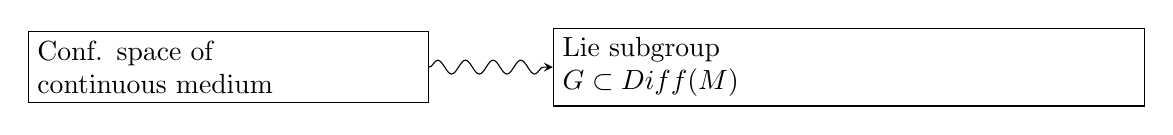
\begin{tikzpicture}[
				node distance=0.65\linewidth,
				]
				\node [text width=0.4\linewidth,rectangle,draw] (lhs) {Conf. space of\\ continuous medium};
				\node [text width=0.6\linewidth, rectangle,draw,right of=lhs] (rhs) {Lie subgroup \\$G \subset Diff(M)$};
				\draw[-stealth,decorate,decoration={snake}] (lhs) -- (rhs);
			\end{tikzpicture}
		}		
		Examples:
		\scalebox{.8}{%		
		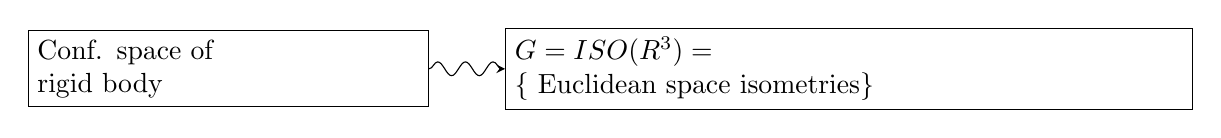
\begin{tikzpicture}[
			node distance=0.65\linewidth,
			]
			\node [text width=0.4\linewidth,rectangle,draw] (lhs) {Conf. space of\\ rigid body};
			\node [text width=0.7\linewidth,rectangle,draw,right of=lhs] (rhs) {$G=ISO(\mathbb{R}^3)=$\\ $\{$
				Euclidean space isometries$\}$};
			\draw[-stealth,decorate,decoration={snake}] (lhs) -- (rhs);
		\end{tikzpicture}
		}
		\scalebox{.8}{%
		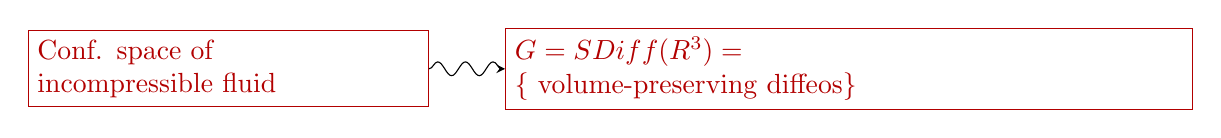
\begin{tikzpicture}[
			node distance=0.65\linewidth,
			]
			\node [text width=0.4\linewidth,red!70!black,rectangle,draw] (lhs) {Conf. space of\\ incompressible fluid};
			\node [text width=0.7\linewidth,red!70!black,rectangle,draw,right of=lhs] (rhs) {$G= SDiff(\mathbb{R}^3)=$\\ $\{$
				volume-preserving diffeos$\}$};
			\draw[-stealth,decorate,decoration={snake}] (lhs) -- (rhs);
		\end{tikzpicture}
		}
	\end{column}%
	\end{columns}
	\pause
	\vfill
	We consider the following setting:
	
	\begin{itemize}%[<+->]
		\item[$\bullet$]2-plectic manifold: 
		\vspace{-1em} 
			$$M=(\mathbb{R}^3,\nu = dx\wedge dy\wedge dz)$$
			\vspace{-.8em}\pause
		\item[$\bullet$]$\infty$-dim. Lie algebra (\emph{ideal fluid velocities}): \vspace{-1em}
			$$\mathfrak{g}:= sdiff_0(\mathbb{R}^3) = \left\lbrace  X \in \mathfrak{X}(\mathbb{R}^3) ~\left\vert~ 
		  		\substack{ div X = 0, \\ \textrm{\emph{ rapidly vanishing at }}\infty} \right\rbrace \right.$$
		  	\vspace{.2em}\pause
		\item[$\bullet$] Multisymplectic Lie algebra action:
			\vspace{-1em} 
			$$\mathfrak{g}= sdiff_0 \hookrightarrow  \mathfrak{X}(\mathbb{R}^3)$$
\end{itemize}		
	\pause
	\vfill
	\begin{center}
	\tcbox[enhanced,frame hidden,borderline={0.5pt}{0pt}{red,dashed}]{	
		\alert{
		\faQuestionCircle \qquad
			{Does $sdiff_0 \circlearrowleft (\mathbb{R}^3,\nu = dx\wedge dy\wedge dz)$ admit an HCMM?}	
		\qquad \faQuestionCircle		
		}
	}
	\end{center}

\end{frame}
\note[itemize]{
	\item We are working in the setting of \emph{geometric continuum mechanics} .\\
		Recall that the configuration space of a continuum object is encoded via diffeomorphisms. In the case of an incompressible fluid is encoded via volume-preserving diffeomorphisms.
	\item (Configution space is the set of spatial displacement of a mechanical systems. These are different from the \emph{physical states}.
	\item Such manifolds are infinite dimensional. Particular caution has to be taken in defining the smooth structure in this case.
	\item However, what really matters in the construction of a moment map is the infinitesimal action, i.e. the Lie algebra. In our case, the infinitesimal action to be considered is via divergence-free vector fields.
	\item (Notation): In the following M will be the 3 dimensional Euclidean Space.
	\item The simple but crucial observation is that the standard volume form on the euclidean space is a multisymplectic form.


}



%---------------------------------------------------------------------------------------------------------------------------------------------------
\begin{frame}{A Hydrodynamical HCMM}\label{frame:hydro2}
	\begin{columns}
		\begin{column}[c]{.5\linewidth}
		  	\begin{itemize}
		  		\item The observables are  $$L= \Omega^1_{\textrm{ham}}(\mathbb{R}^3)\oplus\Omega^0(\mathbb{R}^3)$$
		  		\item \hyperlink{frame:hydromomap-details}{HCMM consists of a pair of functions}:
					\begin{align*}
						f_1 &\colon \mathfrak{g} \rightarrow \Omega^1_{\textrm{ham}}(\mathbb{R}^3) \\
						f_2 &\colon \mathfrak{g}\wedge\mathfrak{g} \rightarrow C^\infty(\mathbb{R}^3)
					\end{align*}	
		  	\end{itemize}
		\end{column}	
	  	\hfill  	
		\begin{column}[c]{.5\linewidth}
  		\includestandalone[width=\textwidth]{Pictures/Figure_Euclid_Trigger}
 	 	\end{column}
 	 \end{columns}


	\pause
\tcbset{colback=white,
	colbacktitle=white,
	colframe=blue!70!black,
	boxrule=1pt,
	colupper=blue!70!black,
	arc=15pt,
	}
	\begin{tcolorbox}[sidebyside,righthand width=.75\linewidth]
		Thm: \cite{Miti2018}
		\tcblower
		\vspace{-1.5em}
		\begin{columns}
		\begin{column}{.6\linewidth}	
		\begin{align*}
		f_1 &= \flat \circ \text{curl}^{-1} 
		%~:~ \mathfrak{g} \to \Omega^{1}_{Ham}(\mathbb{R}^3)
		%\qquad \text{\small ("Biot-Savart law")}
		%\tag{\small"Biot-Savart law"}
		\\
		f_2 &= \Delta^{-1} \circ \delta \circ (f_1 \circ \partial_{CE} +\iota(\cdot)\omega) 
		%~:~ \wedge^2\mathfrak{g} \to C^{\infty}(\mathbb{R}^3)
		%\tag{\small"Coulomb law"}
		\end{align*}		
		\end{column}	
		\begin{column}{.5\linewidth}
			\begin{center}
				\tikz[baseline,remember picture]{\node[rounded corners,
                        fill=orange!5,draw=orange!30,anchor=base]            
            			(base) [rotate=-0,text width=3cm,align=left]{
            				\hyperlink{frame:RiemannianGeneralization}{
            					\footnotesize{
            					Riemannian structure\\\quad plays a crucial role
							}            				
            				}
            			};
            	}		
			\end{center}					
		\end{column}			
		\end{columns}	
	\end{tcolorbox}
	\pause
	\vfill
	\hyperlink{frame:hydro-reinterpretation}{Getting back to hydrodynamics}:
	\begin{tcolorbox}[sidebyside,righthand width=.75\linewidth]
		Thm: \cite{Miti2018}
		\tcblower
		HCMM for $G\circlearrowright(\mathbb{R}^3,\nu)$ induces an ordinary co-mo.map for $G\circlearrowright (LS,\nu^{\ell})$ via \emph{trasgression.}
		\\[.5em]
		\hyperlink{frame:HydroHCMM-reinterpretation}{\alert{\small\emph{(Arnol'd-Marsden-Weinstein hydrodynamical co-momentum map)}}}
		\vfill			
	\end{tcolorbox}


\end{frame}
\note[itemize]{
	\item relation with knot theory: looking at the knot as a fluid configuration with singular vorticity along a knotted tube,
	\item subalgebra of the infinitesimal action of $SDiff(\mathbb{R}^3)$
	\item observe how elements from Riemannian geometry and hodge theory appear in the construction
		\begin{itemize}
			\item $\delta$ codifferential
			\item $\Delta$ Laplacian
			\item $\flat$ $\sharp$  musical isomorphisms
		\end{itemize}

	\item
	Applications:
	\begin{itemize}[<+->]%[<alert@+>]
		\item[\CheckedBox]  Hydrodynamics interpretation: Rasetti-Regge currents as "momenta".
		% is exhibited upon resorting to the Euler equation for perfect fluids.
		\item[\CheckedBox]  Knot theory: reinterpretation of the (Massey) higher order linking numbers in terms of conserved quantities.
		\item[\CheckedBox]  Semiclassical interpretation of the HOMFLYPT polynomial.
	\end{itemize}

	\item other results of the paper: 	
	\begin{itemize}
		\item[\CheckedBox]  Explicit construction of an HCMM for $SDiff_0 \circlearrowright (\mathbb{R}^3,\nu)$ (and generalization to Riemannian homological spheres);
		\item[\CheckedBox]  Hydrodynamics interpretation: proved that this HCMM trasgresses to the standard hydrodynamical co-momentum map of  Arnol'd, Marsden and Weinstein and others; (we recover a quantitity already in use in mechanics)
		% is exhibited upon resorting to the Euler equation for perfect fluids.
		\item[\CheckedBox]  Application to knot theory: reinterpretation of the (Massey) higher order linking numbers in terms of conserved quantities and determined the knot theoretic analogues of first integrals in involution.



	\end{itemize}
	
}
%---------------------------------------------------------------------------------------------------------------------------------------------------



%---------------------------------------------------------------------------------------------------------------------------------------------------
  \begin{frame}{Knot differential forms as observables}\label{frame:hydro3}
	IDEA: Vortex theory approach to knots:
	\begin{itemize}
		\item[\xmark] knots as embeddings $S^1\hookrightarrow \mathbb{R}^3$.
		\item[\cmark] knots as ideal fluid configurations with vorticity concentrated on closed curves
	\end{itemize}
	\pause
	%
	\vfill
  	\begin{columns}
		\begin{column}[c]{.7\linewidth}	
				Let $ L = \cup_{i=1}^n L_i$ be an oriented link in ${\mathbb R}^3$ 
				\\(components $L_i$, $i=1,\dots,n$ required to be  {\it trivial} knots)	
		\end{column}
		\begin{column}[c]{.25\linewidth}
			\centering{
			\includegraphics[width=0.75\linewidth]{./Pictures/Whiteheadlink}
			}
		\end{column}
  	\end{columns}
	%
	\pause
  	\begin{columns}
		\begin{column}[t]{.5\linewidth}	
			\begin{defblock}[Vorticity 2-form]
				$$
				\omega_{L} := \sum_{i=1}^n \omega_{L_i}, \qquad d\omega_L = 0
				$$
				($\omega_{ L_i}$ = \hyperlink{frame:poinduals}{Poincar\'e dual} associated to $L_i$)
			\end{defblock}
		\end{column}
		\begin{column}[t]{.5\linewidth}	
			\begin{defblock}[Velocity 1-form]
				\vspace{-.75em}
				$$
 					v_{ L} = \sum_{i=1}^n v_{L_i}, \qquad \qquad  dv_{L} = \omega_{ L}
				$$
				($v_{L_i} := \omega_{{\mathfrak a}_i}$ = \hyperlink{frame:poinduals}{Poincar\'e dual}  of a disc ${\mathfrak a}_i$ 
				bounded by 	$L_i$ \footnotesize{(Seifert surface)}) 
			\end{defblock}						
		\end{column}
  	\end{columns}
	%
	\pause
	%
	\tcbset{colback=white,
	colbacktitle=white,
	colframe=blue!70!black,
	boxrule=1pt,
	colupper=blue!70!black,
	arc=15pt,
	}
	\begin{tcolorbox}[sidebyside,righthand width=.7\linewidth]
		Thm: \cite{Miti2018}
		\tcblower
		$v_{L}$ is a {\it Hamiltonian 1-form}
		\\[.5em]
		\pause
		\hyperlink{frame:highorderlinking}{\footnotesize{(the same applies to every \emph{"higher velocity $1-form$})}}.
	\end{tcolorbox}	
	 

  
  \end{frame}
  \note[itemize]{
  	\item $G~=~SDiff_0(\mathbb{R}^3)$	(volume-preserving diffeomorphisms) encompasses ambient isotopies of knotted links (interpreted as singular vortices) and Euler evolution
	\item "instead as considering the knot we focus on its complementary"
	\item the context allows to understand certain knot theoretic quantities as hamiltonian forms
	\item $\omega_{ L_i}$ denote the Poincar\'e (or Thom) dual (class) associated to $L_i$: they are 2-forms localized in a 
 cross-section of a  suitable tubular neighbourhood $T_i$ around $L_i$ - with total fibre integral equal to one, or, as currents, 2-forms which are $\delta$-like on $L_i$
 
	\item $v_{L_i} := \omega_{{\mathfrak a}_i}$ is the Poincar\'e dual (class) of a disc ${\mathfrak a}_i$ bounding
$L_i$ (a Seifert surface for the trivial knot $L_i$). Precisely:
$$
\partial {\mathfrak a}_i = L_i, \qquad \qquad dv_{L_i} = d\omega_{{\mathfrak a}_i} = \omega_{L_i} = \omega_{\partial {\mathfrak a}_i},
$$
	\item
		Velocity 1-forms $v_i$ correspond (upon approximation of the associated Euler equation) to the so-called LIA (Linear Induction Approximation) or  {\it binormal evolution}
		of the ``vortex ring" $L_i$ (``orthogonal" to the discs ${\mathfrak a}_i$.
		
	\item Everything is up to choices of tubular neighbourhoods, Seifert surface and specific Poincar\'e dual.	
	
}
%------------------------------------------------------------------------------------------------





%----------------------------------------------------------------------------------------------------------------------------------
\end{document}
%----------------------------------------------------------------------------------------------------------------------------------

%-------------------------------------------------------------------------------------------------------------------------------------------------
%-------------------------------------------------------------------------------------------------------------------------------------------------
	\subsection{Multisymplectic compact group actions on spheres}
	\subcheckpoint	
	\input{defence-spheres}
%-------------------------------------------------------------------------------------------------------------------------------------------------
%-------------------------------------------------------------------------------------------------------------------------------------------------
	\subsection{Gauge transformations, higher Courant algebroids and HCMM}
	\subcheckpoint	
	%+----------------------------------------------------------------------------+
%| SLIDES: 
%| Chapter: Results of the paper with M. Zambon
%| Author: Antonio miti
%| Event: PHD preliminary Defence
%+----------------------------------------------------------------------------+

%- HandOut Flag -----------------------------------------------------------------------------------------
\newif\ifHandout

%- D0cum3nt ----------------------------------------------------------------------------------------------
\documentclass[beamer,10pt]{standalone}   
%\documentclass[beamer,10pt,handout]{standalone}  \Handouttrue  

%- HandOut Flag -----------------------------------------------------------------------------------------
\ifHandout
	\setbeameroption{show notes} %print notes   
\fi

	
%- Packages ----------------------------------------------------------------------------------------------
\usepackage{custom-style}

%--Beamer Style-----------------------------------------------------------------------------------------------
\usetheme{toninus}






%---------------------------------------------------------------------------------------------------------------------------------------------------
%- D0cum3nt ----------------------------------------------------------------------------------------------------------------------------------
\begin{document}
%------------------------------------------------------------------------------------------------


%TITOLO DA AGGIORNARE
%-------------------------------------------------------------------------------------------------------------------------------------------------
%\subsection{Commutative diagram with gauge transformations and HCMM}
%-------------------------------------------------------------------------------------------------------------------------------------------------


%-------------------------------------------------------------------------------------------------------------------------------------------------
\begin{frame}[fragile]{Compatibility between gauge transformations and comoment maps}
	%
	Consider $(M,\omega)$ \alert{symplectic mfd.}
	\only<5-11>{ and \alert{\underline{prequantizable}} ($S^1$-bundle $P$, connection $\theta$)}
	%
	\begin{center}
			\includestandalone[width=.8\textwidth]{Pictures/Frame_BigDiagram_symplectic}
	\end{center}
	%
	\vspace{-2em}
	\begin{minipage}[t][1.7cm][t]{\textwidth}
	\begin{itemize}
		\only<1-4>{
			\item<2-> Given a Symp. mfd. $(M,\omega)$ there is a naturally associated Poisson algebra ...
			\item<3-> .\alert<+>{... and also a Lie Algebroid}.
			\item<4-> A Lie algebroid is a "controlled" $\infty$-dimensional Lie algebra;
		}
		\only<5-6>{
			\item<5-> Prequantization Bundle $S^1\hookrightarrow P \to M$ with connection $\theta$,
			\item<5-> "infinitesimal quantomorphisms" $Q(P,\theta):=\lbrace Y \in \mathfrak{X}(P)~|~ \mathcal{L}_Y \theta =0 \}$.
		}
		\only<7-11>{
		\item<7-> Consider a deformed structure $\tilde{\omega}= \omega + d B$ with $B\in C^\infty(M)$;
		\item<9-> There is a natural isomorphism in the Lie Alg.oids category,
		\item<11-> Considering $\mathfrak{g}\circlearrowleft M$ preserving $\omega$ and $\tilde{\omega}$ ...
		}
		\item<12-> Neglect the prequantization...
		\vspace{-1em} 
			\begin{displaymath}
				\begin{tikzcd}
					\Psi~:&[-1em] C^{\infty}(M)_\omega \ar[r,"\Psi"]& \Gamma(TM\oplus \mathbb{R})_\omega
					\\[-2em]
					& f \ar[r,mapsto] & \binom{\mathscr{v}_f}{f}
				\end{tikzcd}
			\end{displaymath}
	\end{itemize}
	\end{minipage}
	\vfill
	\tcbset{colback=white,
	colbacktitle=white,
	colframe=red!70!black,
	boxrule=1pt,
	colupper=red!70!black,
	arc=15pt,
	}
	\begin{minipage}[t][1.7cm][t]{\textwidth}
	\only<6>{ 
		\begin{tcolorbox}[enhanced,frame hidden,borderline={0.5pt}{0pt}{blue}]
			\color{blue}{
			The left square and right triangles commutes!
			}
		\end{tcolorbox}
	}
	\only<11>{
		\begin{tcolorbox}[enhanced,frame hidden,borderline={0.5pt}{0pt}{blue}]
			\color{blue}{
			The left square and right triangle commute!
			}
		\end{tcolorbox}
	}
	\only<12>{
		\vspace{-.75em}
		\begin{tcolorbox}[enhanced,frame hidden,borderline={0.5pt}{0pt}{blue}]
			\color{blue}{
			The central pentagon commutes!
			}
		\end{tcolorbox}
	\vfill
		\vspace{-.75em}
		\begin{center}
		\tcbox[enhanced,frame hidden,borderline={0.5pt}{0pt}{red,dashed}]{	
			\alert{
			\faQuestionCircle \qquad
				{What happens in the higher (n-plectic) case?}
			\qquad \faQuestionCircle		
			}
		}
		\end{center}
	}
	\end{minipage}
	%
\end{frame}
\note[itemize]{
	\item The horizontal embedding is  $f \mapsto (v_f,f)$;
	\item Vertical maps are also known as \emph{Gauge transformations}
	\item upshot: 
	\begin{enumerate}
		\item 
	\end{enumerate}
}
%-------------------------------------------------------------------------------------------------------------------------------------------------


%-------------------------------------------------------------------------------------------------------------------------------------------------
\begin{frame}[fragile]{Embedding observables $L_\infty$-algebra into Vinogradov $L_\infty$-algebra}
	Consider now $\omega$ \alert{$n$-plectic}
	\vfill
	\begin{center}
		\includestandalone[width=.8\textwidth]{Pictures/Frame_Embedding_Diagram_k-plectic_V1}
	\end{center}
	\vfill
	\only<1-3>{
	\begin{itemize}
		\item<2-> Higher analogue of the Courant algebroid $\rightsquigarrow$ \alert{\emph{Vinogradov algebroid}}
			\begin{displaymath}
			E^n = \left(TM\oplus\bigwedge^{k-1}T^\ast M \right)
			\end{displaymath}
		\item<3->  Vin. alg.oids are $NQ$-manifolds ($L_\infty$-algebroids).
		\\ Associated $L_\infty$-algebra on the graded vector space
		\begin{displaymath}\label{eq:VSpace}
			{\mathcal{V}^k} =
			\begin{cases}
				\mathfrak{X}(M)\oplus \Omega^{n-1}(M)  &\quad k=0,\\
				\Omega^{n-1+k}(M) &\quad -n+1 \leq k < 0.
			\end{cases}
		\end{displaymath}
	\end{itemize}
	}


	\only<4->{
	\begin{thmblock}[Embedding of $L_\infty$-algebras  $\Psi:L_\infty(M,\omega)\hookrightarrow L_{\infty}(E^n,\omega)$\quad \cite{Miti2021}.]
	\begin{itemize}[leftmargin=0pt]
		\item[$\cdot$]<4-> 
			consider the graded vector subspace $\mathcal{A}$
			\begin{displaymath}
			\mathclap{
			{\mathcal{A}^k} =
			\begin{cases}
		\left.\left\lbrace
		\binom{X}{\alpha}\in \mathfrak{X}(M)\oplus \Omega^{n-1}(M)
		~ \right\vert ~
		\iota_X \omega = -d \alpha\right\rbrace
&\quad k=0,\\
				\Omega^{n-1+k}(M) &\quad -n+1 \leq k < 0.
			\end{cases}			
			}
			\end{displaymath}						
		\item[$\cdot$]<5-> 
			restrict the two $L_\infty$-structures to $\pi$ and $\mu$ on $\mathcal{A}$
		\item[$\cdot$]<6->

			$L_\infty(M,\omega) \cong 
				(\mathcal{A},\pi) \color{blue}\cong\color{black}
				(\mathcal{A},\mu) \hookrightarrow
				L_\infty(E^n,\omega)$
	\end{itemize}
	\end{thmblock}
	}
	\only<6->{
		\tikz[overlay,remember picture]
		{
			\node[rounded corners,
                 fill=orange!1,draw=orange!30,anchor=base]            
            	 (base) at ($(current page.east)-(2.25,4)$) [rotate=-0,text width=3cm,align=center] { \footnotesize{\color{red}{
            	 Complete proof\\
            	 \faWarning ~ up to $n\geq 4$! ~ \faWarning 
            	 }}};
		}			
	}

		

\end{frame}
\note{}
%-------------------------------------------------------------------------------------------------------------------------------------------------


%-------------------------------------------------------------------------------------------------------------------------------------------------
\begin{frame}{Compatibility with Gauge transformations}
	Consider now $\omega$ \alert{n-plectic} \quad and \alert{$\tilde{\omega}=\omega + d B$}:
	\vfill
	%
	\begin{center}
		\includestandalone[width=.8\textwidth]{Pictures/Frame_Gauge_Diagram_k-plectic}
	\end{center}	
	%
	\vfill
	%
	

	\begin{itemize}
	\only<1-3>{
		\item<2-> Vinogradov alg.oids w.r.t cohomologous twisting closed forms are isomorphic.
		\item<3-> Induced isomorphism at the level of $L_\infty$-algebras
	}
	\only<4->{
		\item<4-> Consider a Lie algebra action $\mathfrak{g}\to \mathfrak{X}(M)$ admitting HCMM w.r.t $\omega$ and $\tilde{\omega}$
	}
	\end{itemize}

	\vfill
	\tcbset{colback=white,
		colbacktitle=white,
		colframe=blue!70!black,
		boxrule=1pt,
		colupper=blue!70!black,
		arc=15pt,
		}
	\onslide<5->{
	\begin{tcolorbox}[sidebyside,righthand width=.75\linewidth]
		Thm: \cite{Miti2021}
		\tcblower
		\color{blue}
The central square commutes. 
			\\\emph{(On the nose, not "up to homotopies")}.
	\end{tcolorbox}	
		\tikz[overlay,remember picture]
		{
			\node[rounded corners,
                 fill=orange!1,draw=orange!30,anchor=base]            
            	 (base) at ($(current page.east)-(1.75,4)$) [rotate=-0,text width=3cm,align=center] { \footnotesize{\color{red}{
            	 Complete proof\\
            	 \faWarning ~ up to $n\geq 4$! ~ \faWarning 
            	 }}};
		}		
	
	
	}
	

\end{frame}
\note[itemize]{
	\item Our results can be seen as a tiny step toward  undestanding the analogue of prequantization in the setting of multisymplectic geometry (hence field theory).
}
%-------------------------------------------------------------------------------------------------------------------------------------------------




%----------------------------------------------------------------------------------------------------------------------------------
\end{document}
%----------------------------------------------------------------------------------------------------------------------------------





%-------------------------------------------------------------------------------------------------------------------------------------------------


	\thankyouslide

%------------------------------------------------------------------------------------------------

%------------------------------------------------------------------------------------------------




%------------------------------------------------------------------------------------------------
% APPENDIX
%------------------------------------------------------------------------------------------------
\appendix
%-------------------------------------------------------------------------------------------------------------------------------------------------
\section{Complementary Material}
	\input{defence-complementary-material}
	%+----------------------------------------------------------------------------+
%| SLIDES: 
%| Chapter: Bibliography and Figures credit
%| Author: Antonio miti
%| Event: Phd Colloquium - What is ... Geometric mechanics?
%+----------------------------------------------------------------------------+

%- HandOut Flag -----------------------------------------------------------------------------------------
\makeatletter
\@ifundefined{ifHandout}{%
  \expandafter\newif\csname ifHandout\endcsname
}{}
\makeatother

%- D0cum3nt ----------------------------------------------------------------------------------------------
\documentclass[beamer,10pt]{standalone}   
%\documentclass[beamer,10pt,handout]{standalone}  \Handouttrue  

\ifHandout
	\setbeameroption{show notes} %print notes   
\fi

	
%- Packages ----------------------------------------------------------------------------------------------
\usepackage{custom-style}

%--Beamer Style-----------------------------------------------------------------------------------------------
\usetheme{toninus}








%---------------------------------------------------------------------------------------------------------------------------------------------------
%- D0cum3nt ----------------------------------------------------------------------------------------------------------------------------------
\begin{document}
%------------------------------------------------------------------------------------------------


\subsection{References}

%------------------------------------------------------------------------------------------------
% https://en.wikibooks.org/wiki/LaTeX/Bibliographies_with_biblatex_and_biber
\begin{frame}[t,allowframebreaks]{Extended Bibliography}
	%\nocite{*}
	\bibliographystyle{alpha}
	\bibliography{bibfile}
\end{frame}
%------------------------------------------------------------------------------------------------



%------------------------------------------------------------------------------------------------
\begin{frame}[t]{Other aknowledgements}
	\begin{itemize}
		\item Picture - Pendulum 13
			\url{https://andrewjobling.com.au/home-1/everything-okay-becasue-pendulum-swings/}
		\item Picture - Pendulum Phase Space
			\url{https://iopscience.iop.org/article/10.1088/0143-0807/33/2/231}
				\item Picture - Continuum deformation
			\url{https://commons.wikimedia.org/wiki/File:Displacement_of_a_continuum.svg}
		\item Animation - Reidmester moves
			\url{http://realworldmath.tumblr.com/post/57577812688/what-the-hell-is-knot-theory-knot-theory-is-one}
		\item Animation - Bubble rings
			\url{https://www.facebook.com/Nassim.Haramein.official/videos/596203997519126/}
		\item Picture - Whithead link 
			\url{https://en.wikipedia.org/wiki/Whitehead_link}
		\item Picture - Gauss linking number 
			\url{https://www.maths.ed.ac.uk/~v1ranick/papers/ricca.pdf}
		\item Picture - Borromean Rings
			\url{https://en.wikipedia.org/wiki/Borromean_rings}	
	\end{itemize}
\end{frame}
\note[itemize]{
	\item
}
%------------------------------------------------------------------------------------------------



%------------------------------------------------------------------------------------------------
\end{document}
%------------------------------------------------------------------------------------------------










%------------------------------------------------------------------------------------------------
\end{document}

